\chapter{Dust Attack}
Gli obiettivi principali di questa tesi sono:
\begin{itemize}
\item Definire il Dust Attack, spiegandone le conseguenze e le possibili contromisure;
    \item Presentare delle statistiche generali su come venga speso il dust, in particolare mostrare se e quanto possa essere efficace un Dust Attack mostrando gli effetti del dust sulla de-anonimizzazione degli address e dei relativi wallet;
    \item Descrivere due pattern interessanti che sono stati trovati e che potrebbero rappresentare casi di Dust Attack.
\end{itemize}
Il Dust Attack è una nota tecnica che sfrutta gli importi dust. È importante quindi spiegare cosa sia il dust e in generale quali possano essere i suoi possibili impieghi.
\section{Dust}
%Una transazione in generale può essere multi-input e multi output: sono presenti quindi più address %paganti e/o più address riceventi, generalmente l'importo totale di input non viene speso in output %ma parte di esso viene dato ai miners come fee. Formalmente la fee, raccolta dai miners come %ricompensa per includere la transazione in un blocco, è definita come:
%\begin{center}
 %   $fee = \sum_{inputs} importo(input_i) - \sum_{outputs} importo(output_i)$
%\end{center}
\section{Usi del dust}
\subsection{Satoshi Dice}
Satoshi Dice è un noto "gioco di scommesse basato su blockchain" nato nell'Aprile 2012 \cite{SD}. A differenza dei tradizionali software di gioco online, le scommesse con Satoshi Dice possono essere inviate senza accedere al sito Web né eseguire alcun software client. Per giocare, viene effettuata una transazione Bitcoin a uno degli address resi pubblici da Satoshi Dice, ciascuno con pagamenti diversi. Tutti gli address resi pubblici da Satoshi Dice sono vanity address, tutti gli address infatti presentano il prefisso \textbf{1dice}. Un vanity address in generale è un address Bitcoin con le stesse funzionalità di qualsiasi altro address ma presenta una stringa personalizzata contenente una parola o un messaggio comprensibili alle persone. Un esempio di vanity address è 1BoatSLRHtKNngkdXEeobR76b53LETtpyT, che contiene la parola Boat. Ogni address \textbf{1dice} presenta probabilità diverse di vincere la scommessa, generalmente minore è la probabilità maggiore è il compenso che si ottiene da una vincita. Per esempio 1dice1e6pdhLzzWQq7yMidf6j8eAg7pkY offre una probabilità dello 0,0015\% di vincere 64 000 volte la puntata originale. Per determinare se una scommessa è vincente o perdente, Satoshi Dice utilizza genera un numero casuale, il quale viene assegnato al giocatore. Il servizio successivamente utilizza una combinazione dell'hash della transazione della scommessa ed esegue un hash SHA2 a 512 bit prendendo come input l'hash della transazione utilizzando un segreto sconosciuto al giocatore. I primi quattro byte dell'output diventano il numero che determina se il giocatore abbia vinto la scommessa.

Il servizio, dopo aver determinato le scommesse vincenti e quelle perdenti, invia una transazione in risposta con il pagamento al vincitore e restituisce un sinoglo satoshi ai giocatori perdenti per comunicare loro la perdita.
\subsection{OP RETURN}
Le transazioni in Bitcoin sono molto più complesse \cite{script} di come descritte nel capitolo precedente \ref{Transazioni}, non contengono solo valori come address e importo ma includono anche del codice, in particolare ogni transazione comprende anche degli script che descrivono come la persona successiva che desidera spendere i bitcoin trasferiti possa accedervi. 

Bitcoin utilizza un sistema di script Forth-like, basato su stack e non Turing-completo; questa scelta di evitare i loop è intenzionale in quanto impedisce possibili cicli infiniti. 

Gli script \cite{opcode} in Bitcoin sono:
\begin{itemize}
    \item Senza stato: non esiste uno stato prima dell'esecuzione di uno script né viene salvato dopo l'esecuzione.
    \item Deterministici: uno script viene eseguito alla stessa maniera in ogni sistema.
    \item Semplici e compatti: le istruzioni, gli OP\_CODE, sono codificate in un singolo byte. In totale ci sono 75 istruzioni funzionanti e 15 disabilitate.
\end{itemize}
Gli OP\_CODE in Bitcoin comprendono diverse categorie:
\begin{itemize}
    \item aritmetica di base: OP\_ADD, OP\_SUB;
    \item controllo di flusso: OP\_IF, OP\_ELSE;
    \item logica bit a bit: OP\_EQUAL;
    \item gestione stack: OP\_DROP, OP\_SWAP;
    \item hashing: OP\_SHA1, OP\_SHA256;
    \item verifica firma o multifirma: OP\_CHECKMULTISIG.
\end{itemize}

Le transazioni Bitcoin non forniscono un campo dove si possono salvare dati arbitrari \cite{arbdata}. Tuttavia, gli utenti hanno ideato vari modi creativi per codificare i dati nelle transazioni. Questi metodi però modificavano il protocollo di transazione rendendo inspendibili gli output così generati. Il problema è che questi output non erano facilmente distinguibili dagli altri quindi in nodi della rete dovevano salvarli nei loro UTXO set.

L'UTXO(Unspent Transaction Output) set è l'insieme degli output riscattabili di tutte le transazioni della blockchain. Per essere valida, una transazione deve
utilizzare solo elementi dell'UTXO come input.

Poiché questo set, per motivi di efficienza, è solitamente memorizzato nella RAM \cite{utxo} questa pratica influiva negativamente sul consumo di memoria dei nodi \cite{stresstest}.

Per risolvere tale problema nel 2014 è stato reso standard il codice OP\_RETURN \cite{opreturnstandard} . Questo OP\_CODE era presente fin dalla nascita di Bitcoin, però era considerato non-standard proprio perchè la scrittura di dati arbitrati sulla blockchain non viene considerata una buona pratica. Questo codice permette di segnare un output della transazione come non valido, quindi successivamente non potrà essere speso.

Siccome gli output con questo OP\_CODE non possono essere spesi, possono essere rimossi dall'UTXO set. In questo modo OP\_RETURN risolve il problema del consumo di memoria spiegato precedentemente. Il limite iniziale per la memorizzazione dei dati con questo codice era pianficato per essere di 80 byte, ma inizialmente ne furono concessi 40(versione 0.9.0).  La versione 0.11.0 \cite{v11} ha esteso il limite di dati a 80 byte e la versione 0.12.0 \cite{v12} fino a un massimo di 83 byte. 

Come riportato in \cite{OP_RETURN} esistono diversi protocolli che sfruttano OP\_RETURN. Di solito, un protocollo è identificato dai primi byte di metadati allegati all'OP RETURN, ma il numero esatto di byte può variare da protocollo a
protocollo. 

Questi protocolli possono essere divisi in categorie tra le quali:
\begin{itemize}
    \item Risorse: protocolli che sfruttano l'immutabilità della blockchain per certificare la proprietà, lo scambio e, infine, il valore dei beni del mondo reale. I metadati nelle transazioni vengono utilizzati per specificare ad es. il valore del bene, il importo del bene trasferito, il nuovo proprietario, ecc;  
    \item Atti notarili: protocolli per la certificazione della proprietà di un documento. Un utente può pubblicare l'hash di un documento in una transazione, e in questo modo può provarne l'esistenza e l'integrità;
    \item Arte digitale: protocolli per la dichiarazione dei diritti di accesso e di copia di arti digitali, come ad es. foto o musica.
\end{itemize}
%``"
In generale salvare dati sulla blockchain di Bitcoin non è una buona pratica, infatti anche la documentazione ufficiale di Bitcoin sconsiglia questo utilizzo \footnote{Le note di rilascio di  Bitcoin Core versione 0.9.0 affermano che: “Storing arbitrary data in the blockchain is still a bad idea; it is less costly and far more efficient to store non-currency data elsewhere.”}.
\section{Dust Attack}
Come visto nel capitolo precedente \ref{Anonimato} esistono delle euristiche che possono essere sfruttate per effettuare determinati attacchi in grado di violare l'anonimato di Bitcoin. L'attacco che verrà approfondito in questa tesi viene denominato \textbf{Dust Attack}. 

L'euristica utilizzata da questo tipo di attacco è la regola degli input multipli:
\begin{center}
    ``\textit{In una transazione multi-input tutti gli address appartengono allo stesso utente}"
\end{center}
L'obiettivo del Dust Attack è la de-anonimizzazione del proprietario di un wallet, in particolare l'attaccante vuole scoprire quali address appartengano allo stesso wallet, così da ottenere un'importante informazione che può essere utilizzata per effettuare altri attacchi più elaborati e molto più pericolosi. Nel paragrafo \ref{Conseguenze} verrà approfondito questo aspetto.

Il Dust Attack deriva il proprio nome dall'impiego del dust, infatti il dust, nelle transazioni standard, non è mai speso singolarmente ma viene sempre unito ad altri importi. L'attaccante quindi, come mostrato in figura \ref{fig:Dust_attack}, invia centinaia, o migliaia, di importi dust ad address diversi confidando che vengano spesi successivamente in una nuova transazione insieme ad altri address. Se ciò avviene l'attaccante riesce a collegare questi address e capire che appartengono, con una certa probabilità, allo stesso utente.\\ 

Il Dust Attack ad un primo sguardo potrebbe sembrare particolarmente costoso, proprio perchè invia tanti importi ad address differenti, ma se analizziamo il valore in euro di un singolo satoshi, ci accorgiamo subito che il costo è relativo; soprattutto se l'obiettivo finale è il furto dei bitcoin delle vittime. Infatti abbiamo che:
\begin{center}
    1 satoshi = 0.00016 € (in data 16/11/2022) 
\end{center}

Questo significa che 1 singolo satoshi vale meno di 1 centesimo, quindi se un attaccante genera una transazione con 1000 output dust e manda a ciascun address 1 satoshi, in totale spende poco più di un euro, escludendo la fee.  
\begin{figure}[h!]
    \centering
    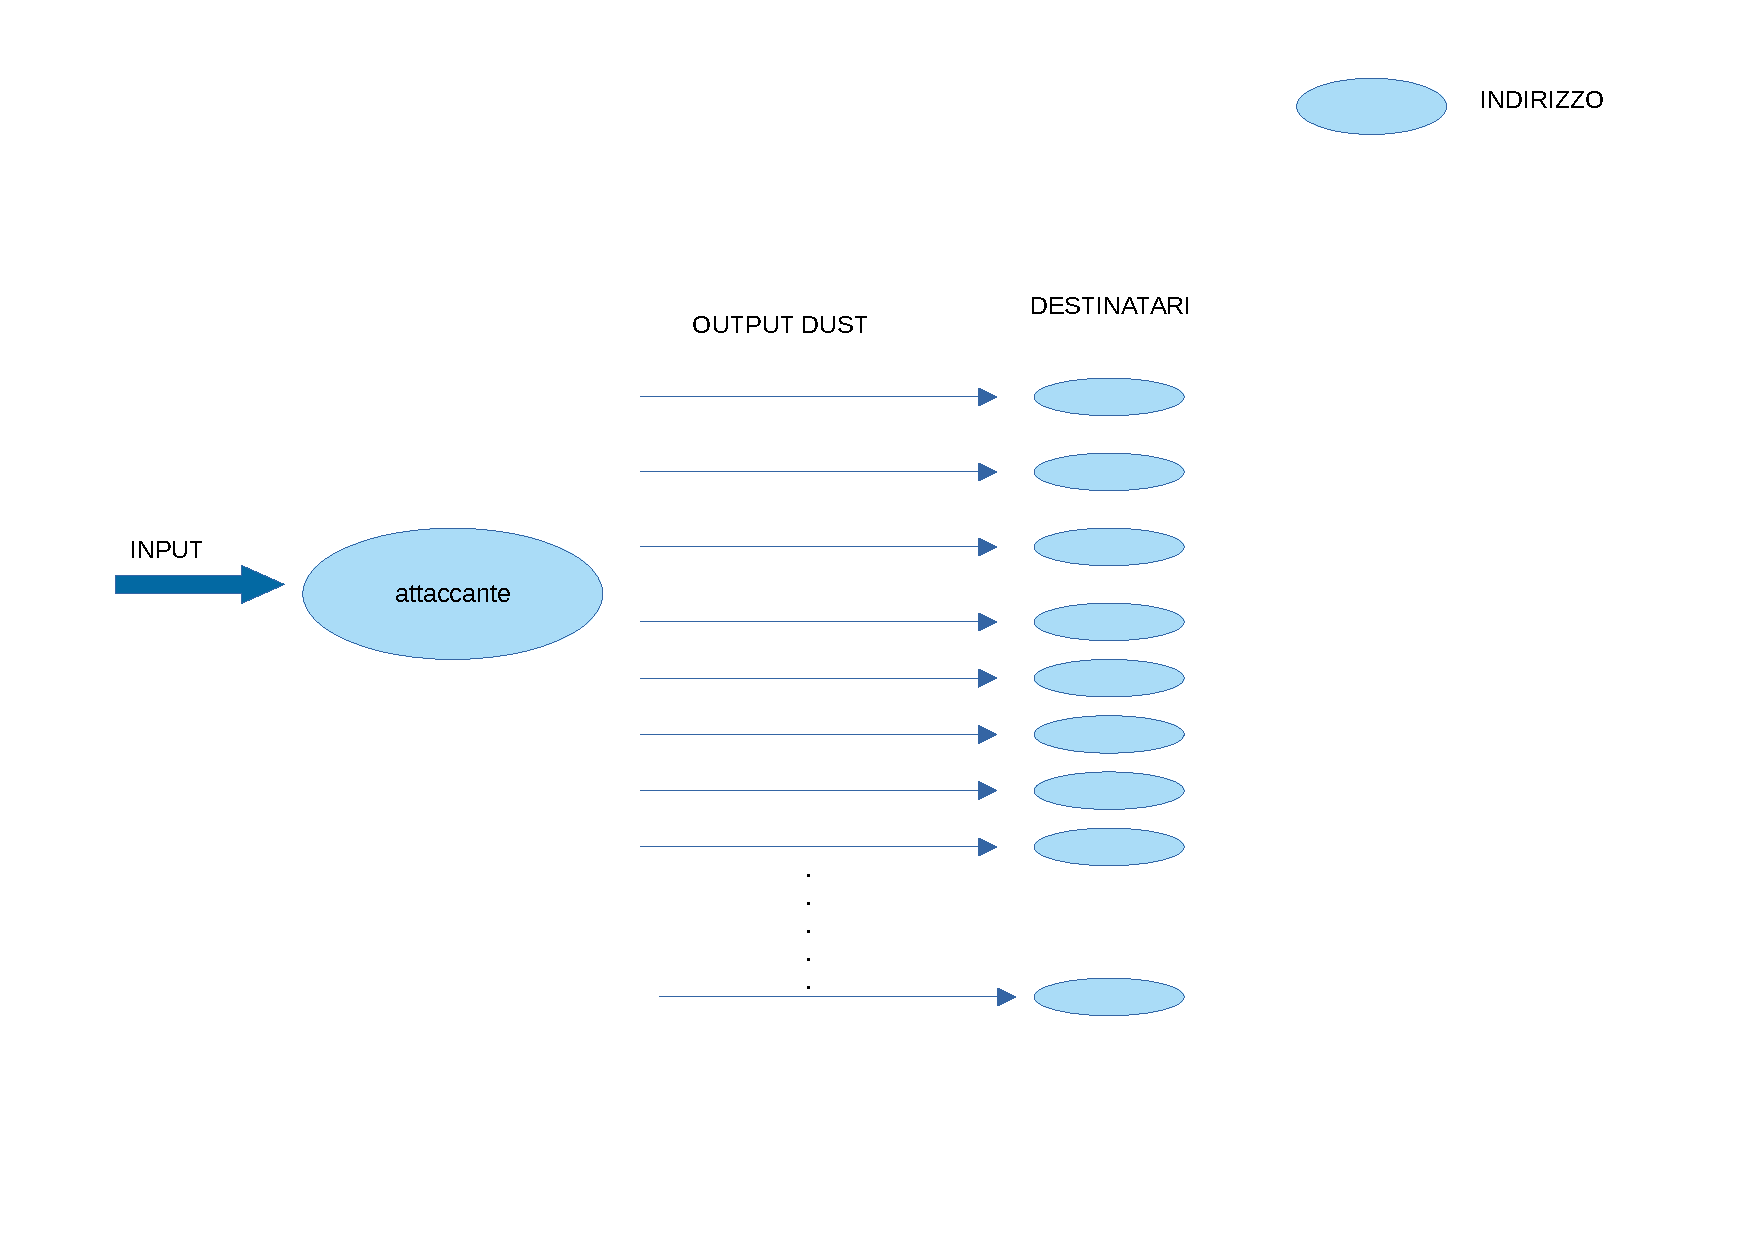
\includegraphics[scale=0.5]{Images/dust_attack.pdf}
    \caption{Schema Dust Attack}
    \label{fig:Dust_attack}
\end{figure}
\FloatBarrier
Una volta effettuato l'attacco possono esserci due possibili esiti: 
    \begin{enumerate}
        \item attacco di successo;
        \item attacco fallito;
    \end{enumerate}
Nel primo caso, mostrato in figura \ref{fig:success}, la vittima genera una transazione in cui spende l'importo dust ricevuto insieme ad almeno un altro dei suoi address. 

Questi address quindi sono collegati tra loro ed è possibile capire che appartengano ad uno stesso utente. Se l'attaccante successivamente scopre le informazioni personali, come nome o email, del proprietario di uno di questi address automaticamente scopre che tutti gli altri address hanno lo stesso proprietario; inoltre è possibile tracciare l'attività di un singolo utente e non solo di un address singolo.\\
\begin{figure}[h!]
    \centering
    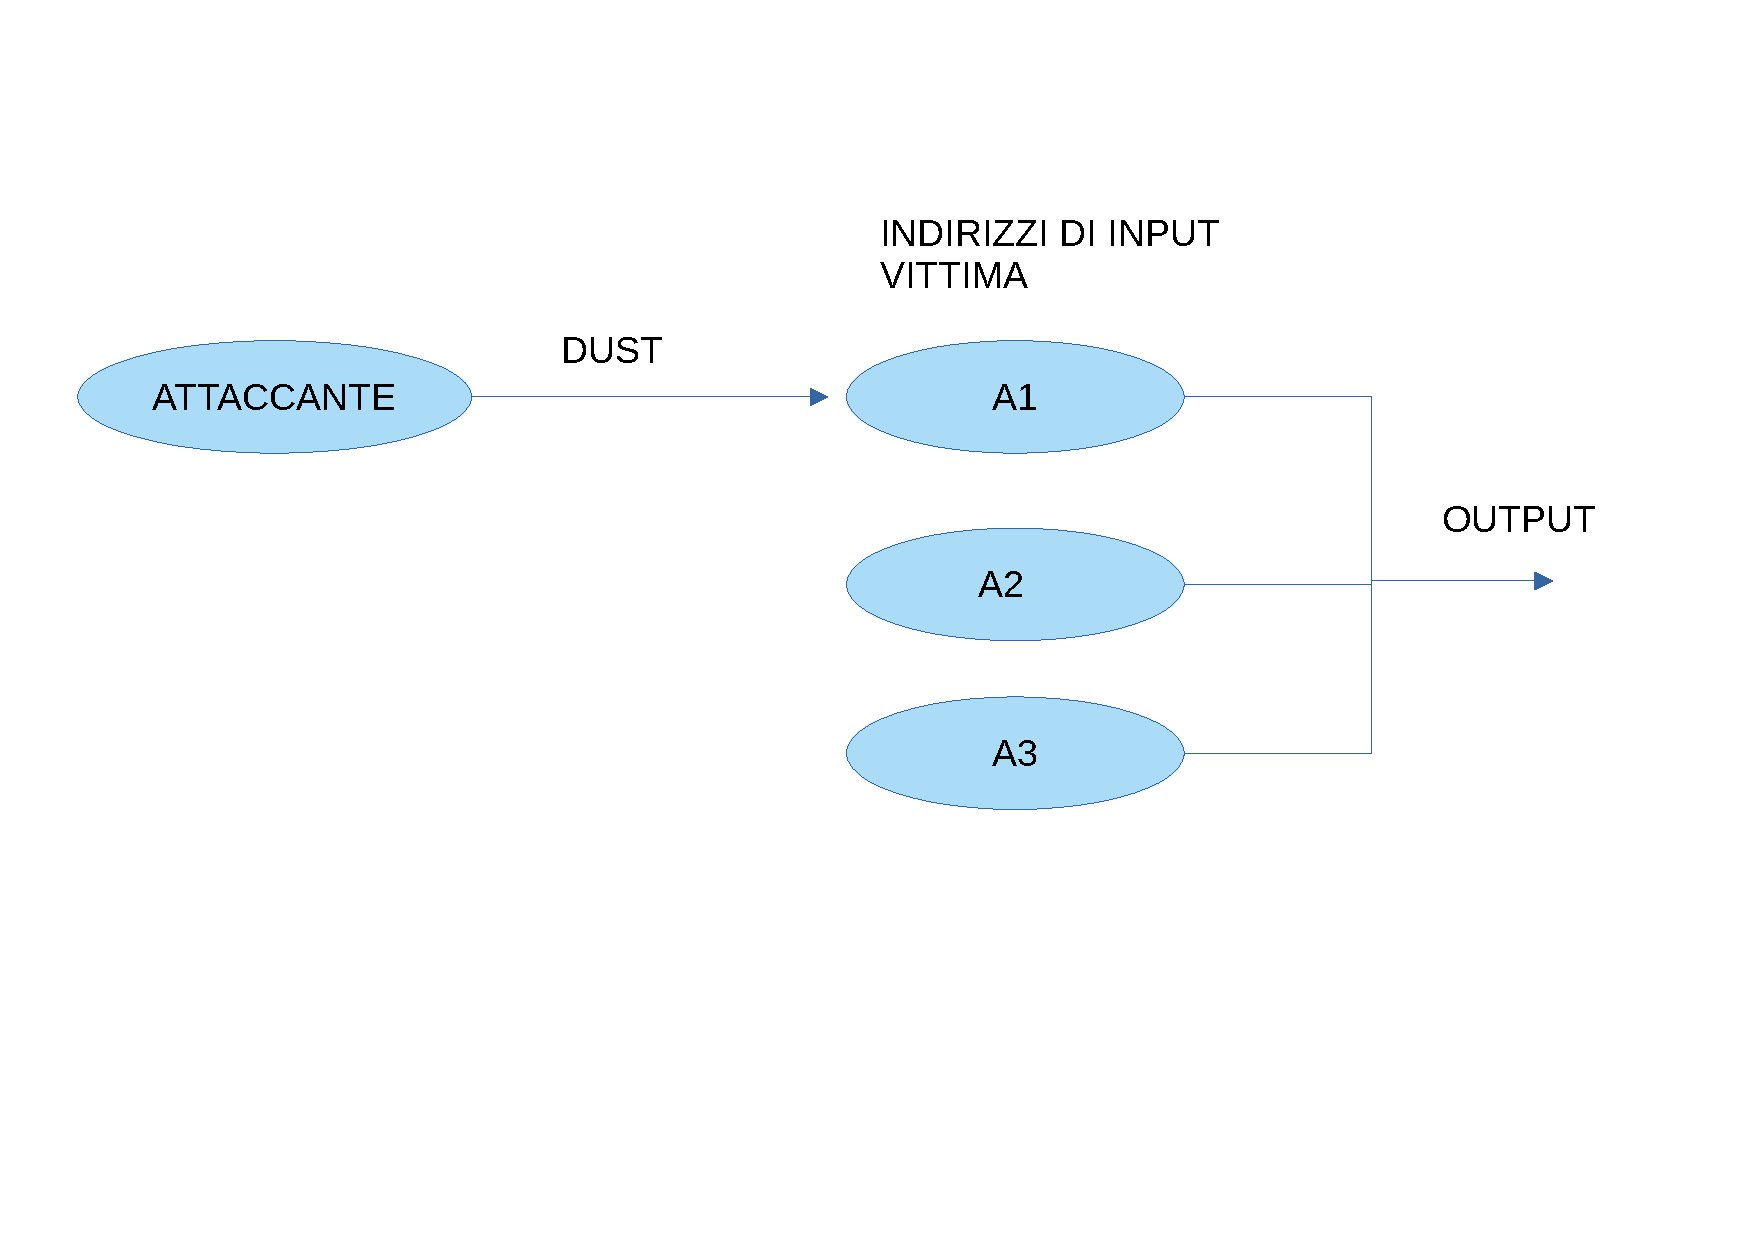
\includegraphics[scale=0.5]{Images/successo.pdf}
    \caption{Schema Attacco di Successo}
    \label{fig:success}
\end{figure}
\FloatBarrier
Esistono invece due possibili motivi per cui un Dust Attack possa fallire. In figura \ref{fig:fallito} vengono schematizzati questi due possibili esiti.

Nel primo schema la vittima spende il dust ricevuto, ma utilizza un solo address di input, l'attaccante quindi non è in grado di ricavare alcuna informazione. Nel secondo schema invece la vittima non spende il dust, troncando sul nascere l'attacco. 
\begin{figure}[h!]
    \centering
    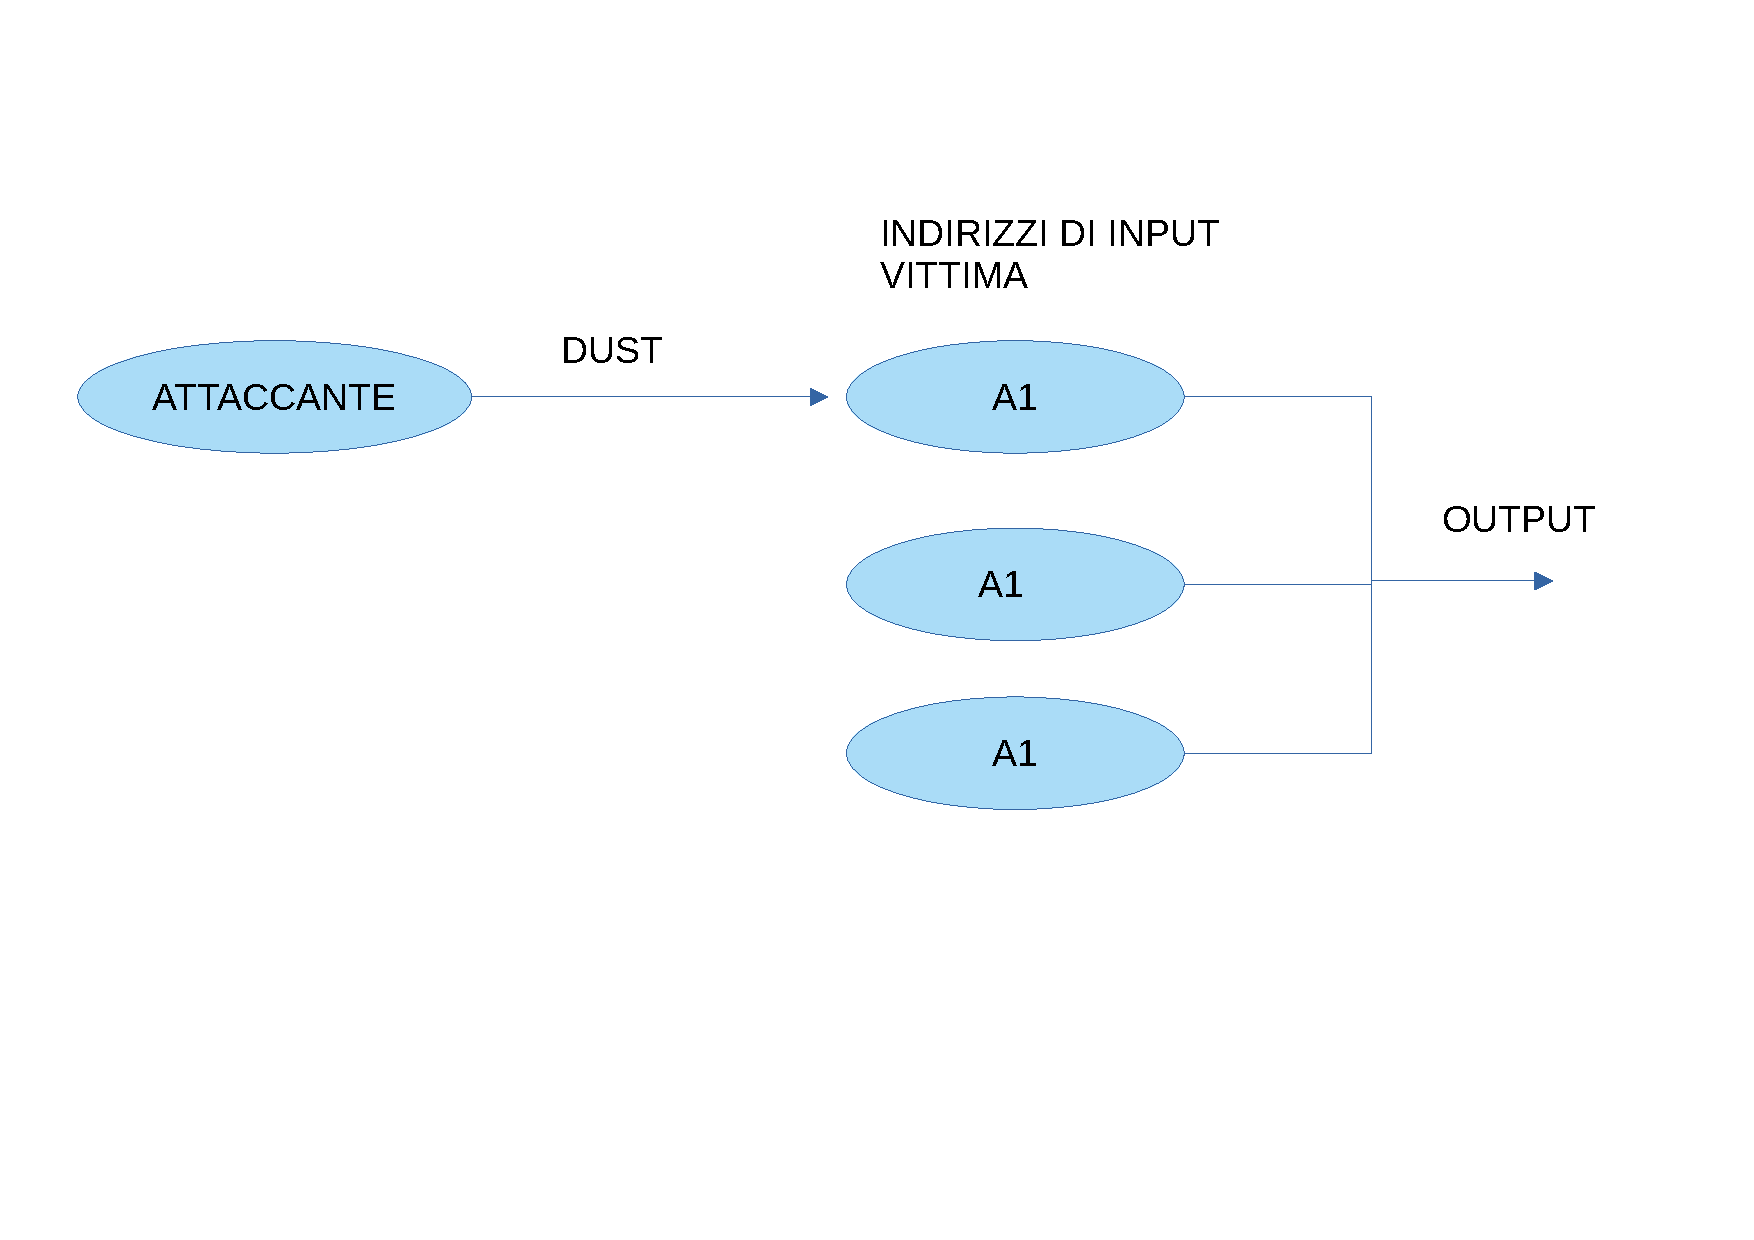
\includegraphics[scale=0.5]{Images/fallimento.pdf}
    \caption{Schema Attacco Fallito}
    \subcaption{La vittima spende il dust(sopra) con un solo address. La vittima non spende il dust(sotto)}
    \label{fig:fallito}
\end{figure}
\FloatBarrier
Il Dust Attack in generale risulta più efficace soprattutto contro gli address che hanno un bilancio complessivo pari a zero proprio perché obbliga la vittima a spendere la cifra ottenuta con altri suoi address diversi.\\

È importante notrare che il Dust Attack non permette di rubare fondi di altri utenti né permette di scoprire le informazioni personali, per esempio nome e cognome, della vittima ma permette di ricavare un'importante informazione che può essere usata in seguito per effettuare attacchi elaborati e più pericolosi.
\subsection{Conseguenze}\label{Conseguenze}
Come detto in precedenza questa tipo di de-anonimizzazione di per sé non costituisce un problema. Può diventarlo se viene usata come mezzo per altri tipi di attacchi. In generale il Dust Attack non per forza è legato a phishing o estorsioni ma potrebbe essere usato dalle autorità per tenere traccia degli utenti ed eventualmente rilevare attività illegali.

Infatti una volta otteuto un cluster di address riesco a tracciare l'attività di un singolo utente e non più di un singolo address. Le autorità potrebbero notare che certi utenti interagiscono con address legati a mercati neri, e quindi indagare ulteriormente per scoprire l'identità di queste persone. Uno dei punti fondamentali è legare informazioni personali, come e-mail, nome ed altro, a address Bitcoin. In molti casi sono gli utenti stessi che pubblicano sui forum i loro address, in altre situazioni invece è possibile sfruttare gli exchange come Coinbase.\\

Gli exchange sono servizi che permettono lo scambio tra criptovalute e valute tradizionali basandosi sul valore di mercato della criptovaluta. In exchange come Coinbase è necessario creare un account fornendo informazioni personali come nome, cognome, email ed altro e, una volta registrati, viene creato un wallet associato a quel particolare account. Siccome gli exchange sono esposti ad attacchi hacker molti utenti trasferiscono i loro bitcoin su address appartenenti a software wallet, per esempio Wasabi Wallet.\\

Una volta che un utente effettua un deposito dal wallet, vittima di Dust Attack, ad un account exchange ecco che l'attaccante collega gli address al proprietario. Una volta ottenuta l'identità del proprietario l'attaccante può eseguire elaborati attacchi di phishing oppure può estorcergli il denaro minacciandolo di rivelare a tutti l'informazione ottenuta.\\ 

Il Dust Attack però non risulta particolarmente difficile da contrastare, nel paragrafo successivo verranno mostrati due metodi per difendersi da questo tipo di attacco.
\subsection{Contromisure}
Due metodi per contrastare il Dust Attack sono:
    \begin{enumerate}
        \item non spendere l'importo dust ricevuto; 
        \item utlizzare servizi di ``dust collecting". 
    \end{enumerate}
    
La prima soluzione, semplice ed efficace, permette di troncare l'attacco sul nascere. Infatti se il dust non viene speso l'attaccante non potrà mai collegare address diversi dello stesso utente. 

Questo metodo può esserre effettuato in diversi software wallet; per esempio Samurai Wallet \footnote{fonte:\url{https://twitter.com/samouraiwallet/status/1055345822076936192?lang=en}}, nel 2018, consigliò ai suoi utenti, possibili vittime di Dust Attack,  di contrassegnare come "do not spend" l'output dust ricevuto.\\

La seconda soluzione riguarda i servizi di ``dust collecting", per esempio Dust-B-Gone \cite{Dbg}.
Dust-B-Gone, ideato da Peter Todd già nel 2012, era un servizio che permetteva di disfarsi del dust. L'obiettivo era di non lasciare il dust ricevuto come UTXO ma di spenderlo e trasformarlo in fee per i miner.

Il programma generava un'unica transazione alla quale potevano partecipare più utenti, ogni utente inseriva tra gli input il proprio importo ricevuto così da potersene liberare. Allo stesso tempo questo servizio proteggeva gli utenti da una possibile de-anonimizzazione, poichè indirizzi diversi potevano appartenere ad utenti diversi. Un attaccante quindi non avrebbe mai potuto collegare questi address, o comunque avrebbe ricavato una falsa informazione.
Purtroppo questo servizio è stato chiuso nel 2016 per vari motivi tra cui il suo poco utilizzo \footnote{fonte: \url{https://twitter.com/SamouraiWallet/status/1293659938422652935}} . 